De esta forma, se corroboró mediante observación que la imagen mostrada al usuario

\begin{figure}[H]
\centering
    	\begin{subfigure}{0.49\textwidth}
        	\centering
        	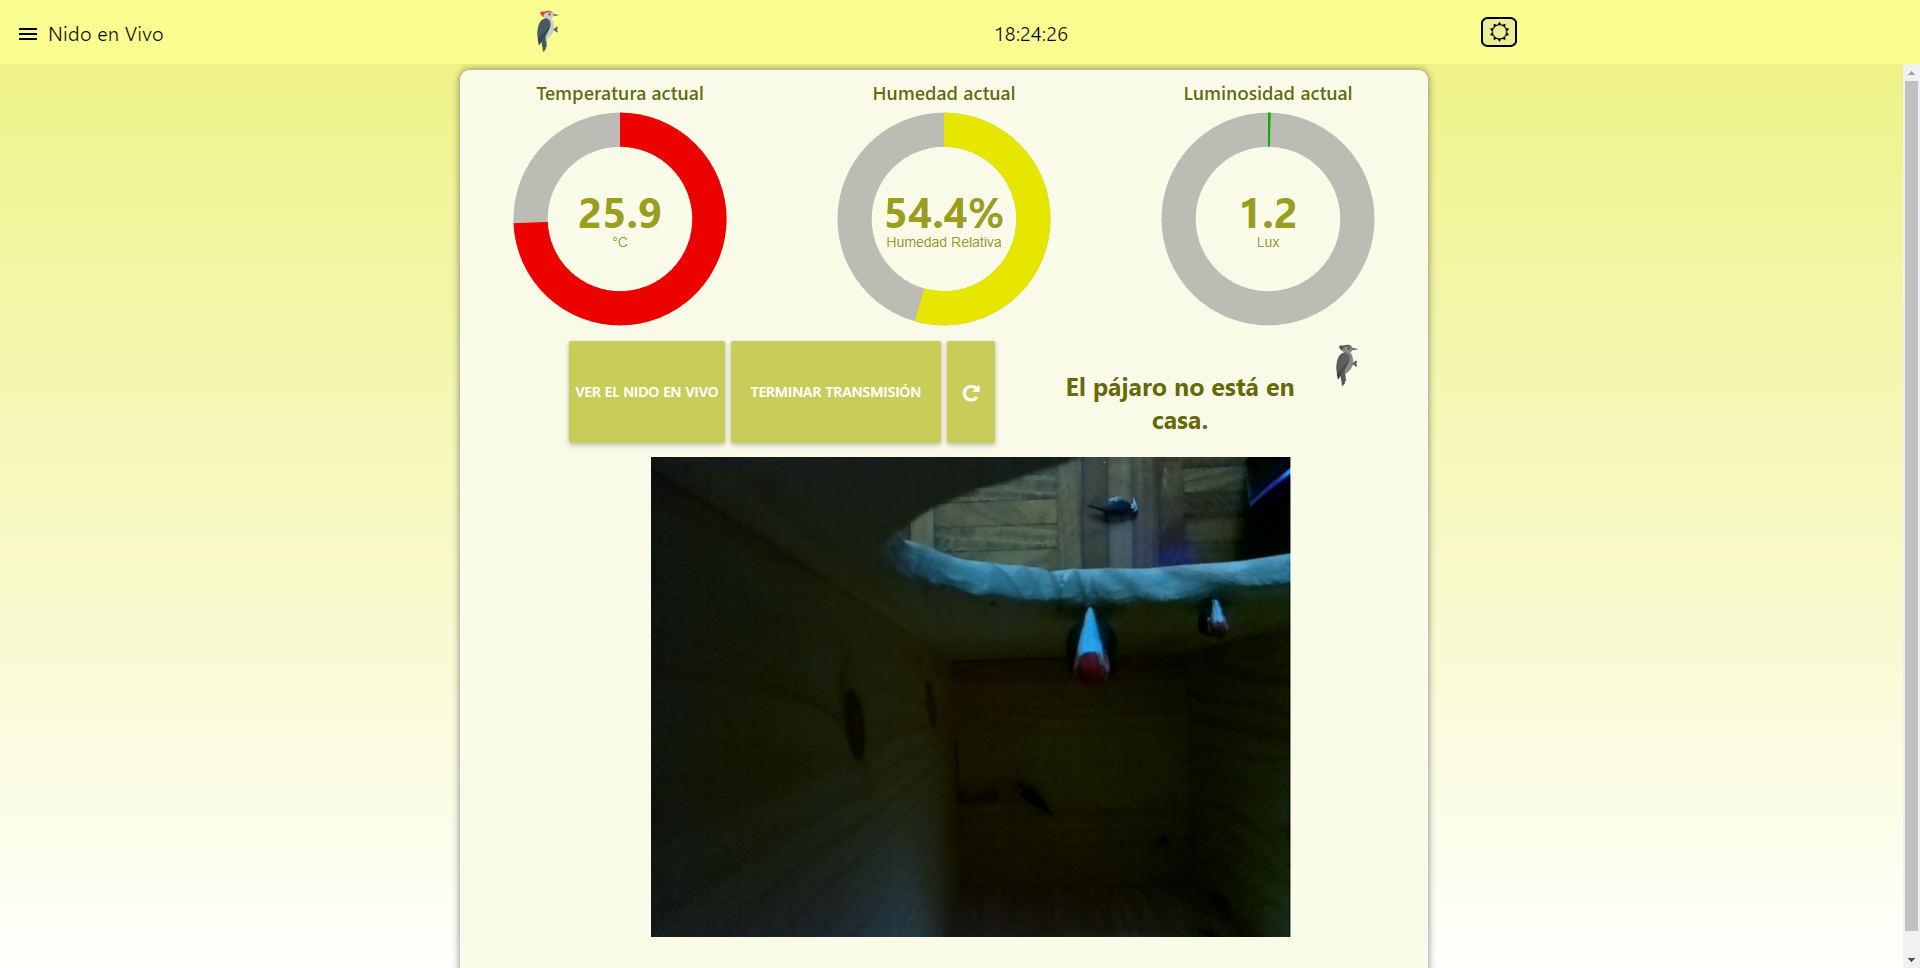
\includegraphics[width=\linewidth]{ImagenesValidacion del prototipo/t-int-fun-04-12-1}		
			\caption{Vista de la transmisión en vivo del nido.}
        \end{subfigure}\hfill
        \begin{subfigure}{0.49\textwidth}
        	\centering
        	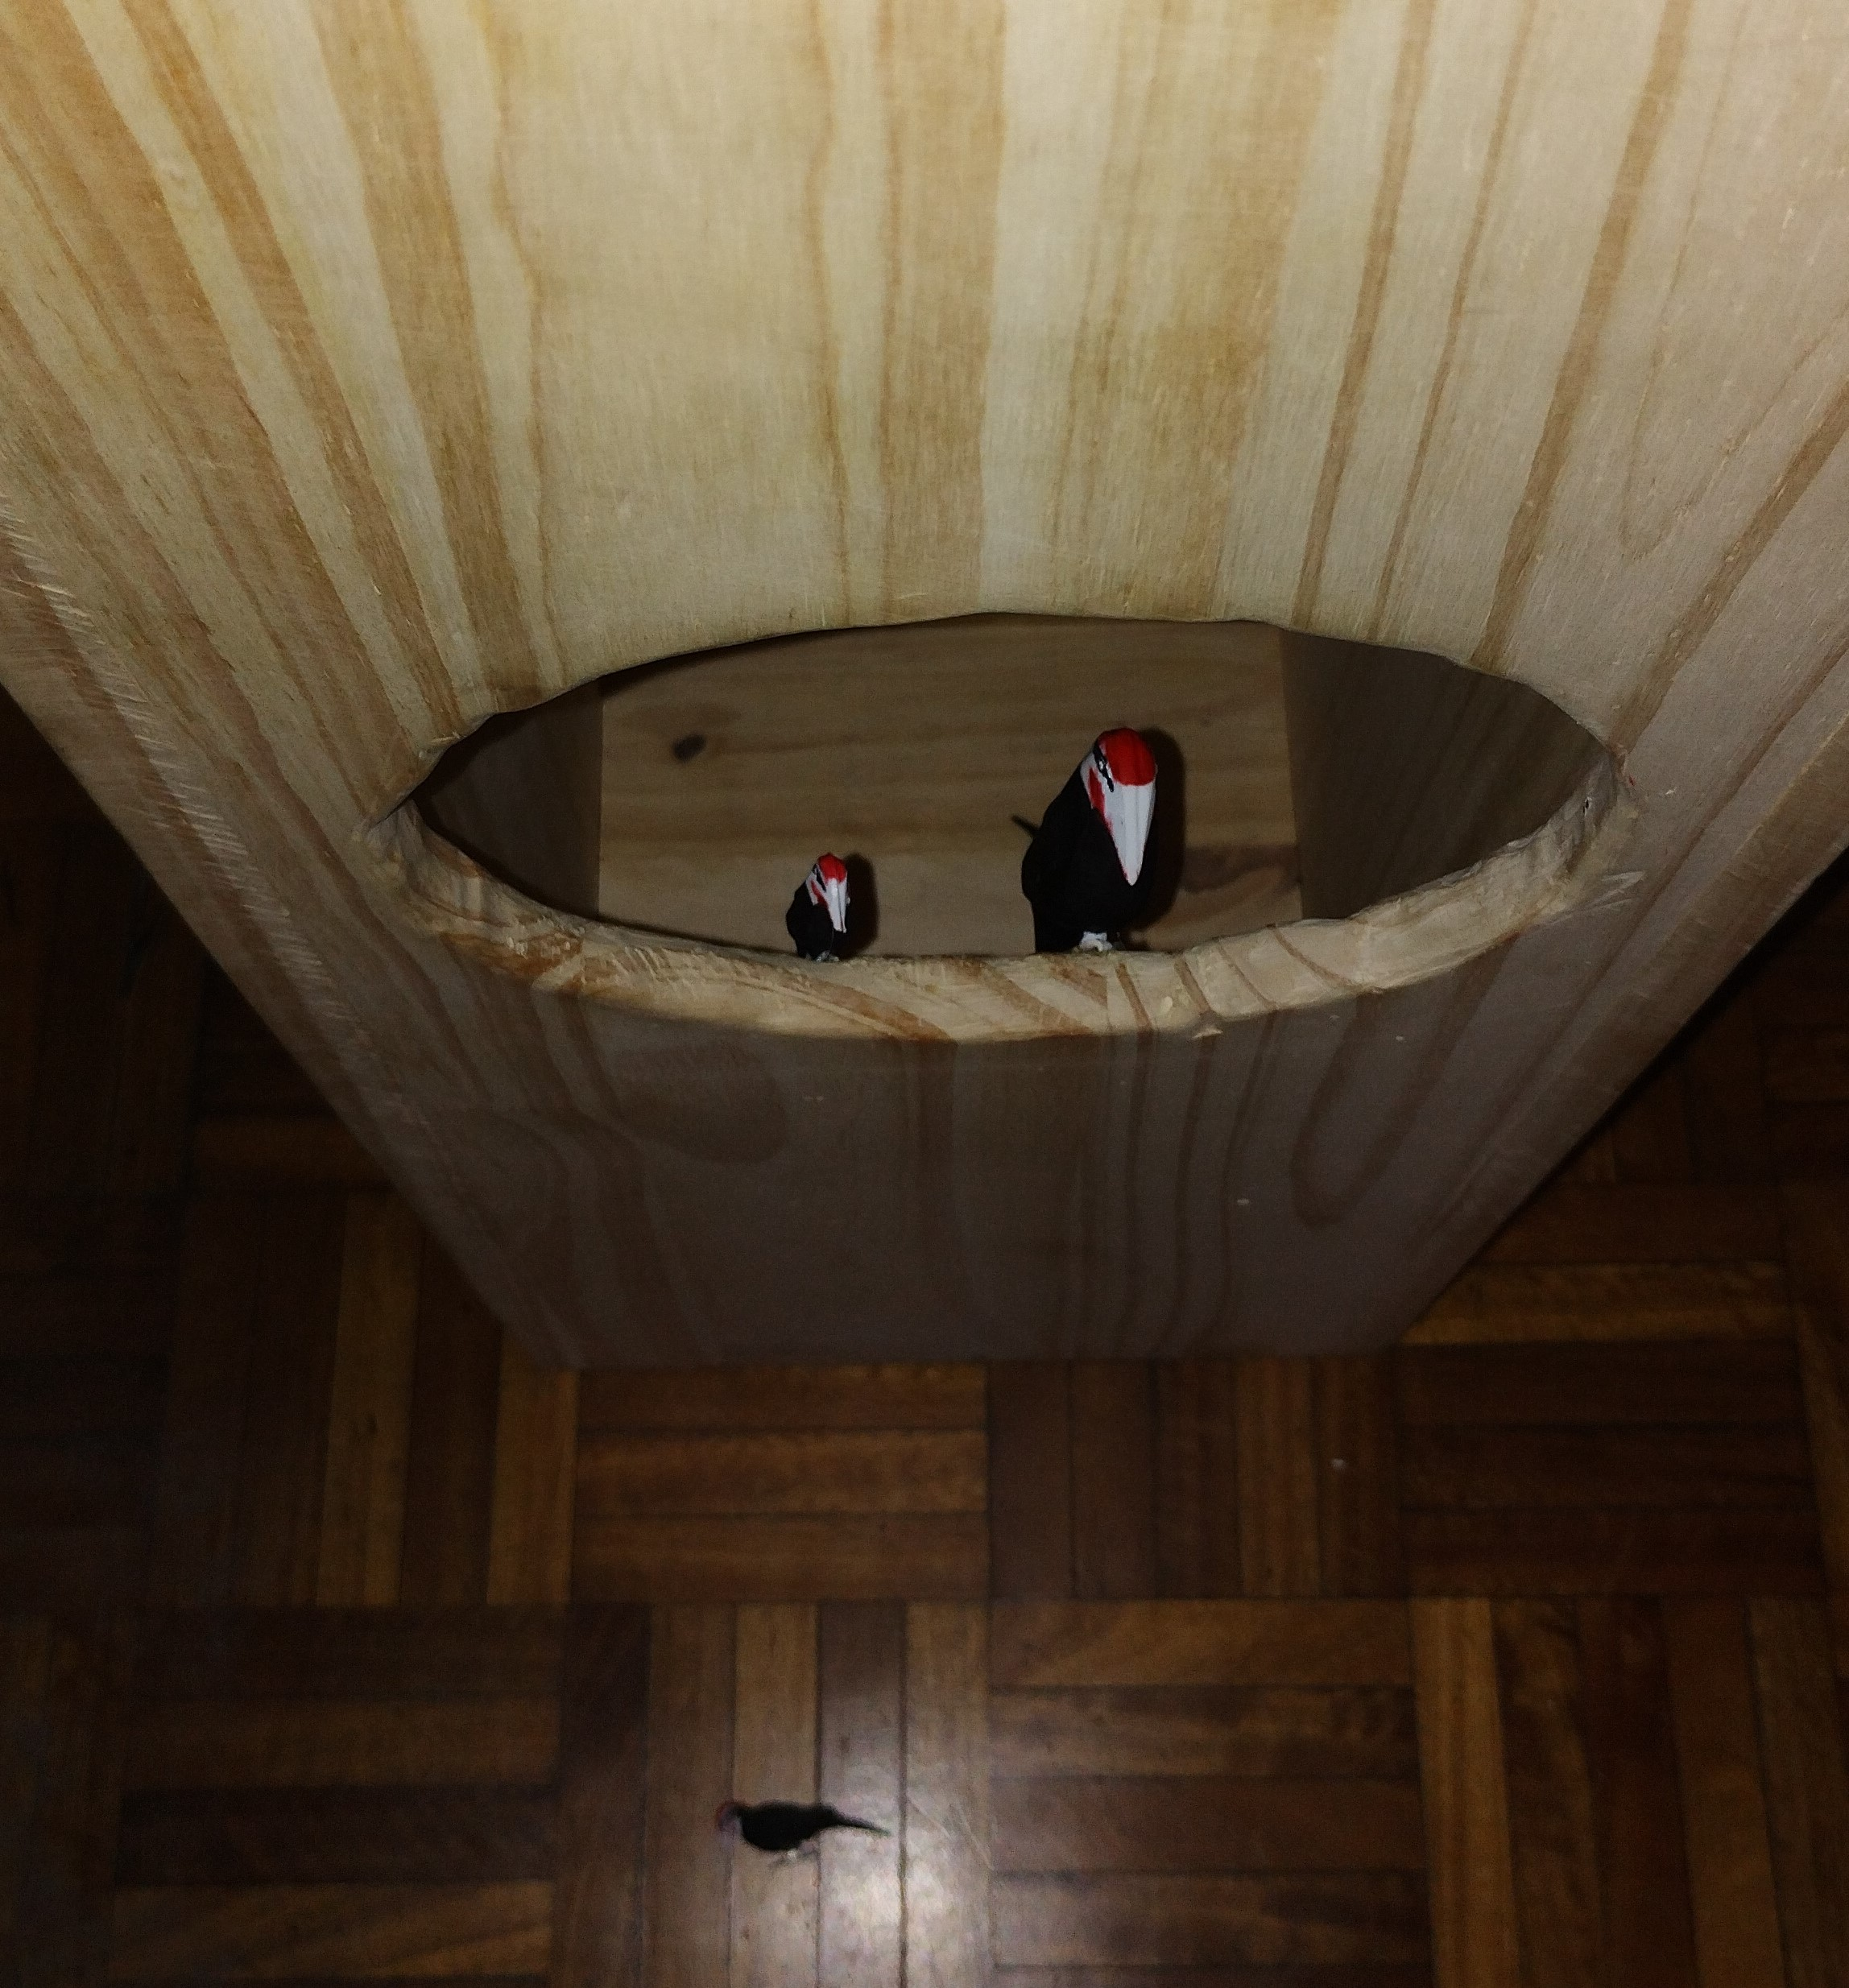
\includegraphics[width=0.5\linewidth]{ImagenesValidacion del prototipo/t-int-fun-04-12-2}
        	\caption{Imagen del exterior del nido en el momento de la trasmisión.}
        \end{subfigure}
	\caption{Validación de funcionalidad \textit{T-INT-FUN-04} y \textit{T-INT-FUN-12}.}
\end{figure}


Se dispuso del banco de pruebas \#1 para analizar la aplicabilidad de \textit{T-RAM-SEG-01}. El acceso tanto a la interfaz gráfica para el usuario como la desarrollada

\begin{figure}[H]
\centering
    	\begin{subfigure}{0.49\textwidth}
        	\centering
        	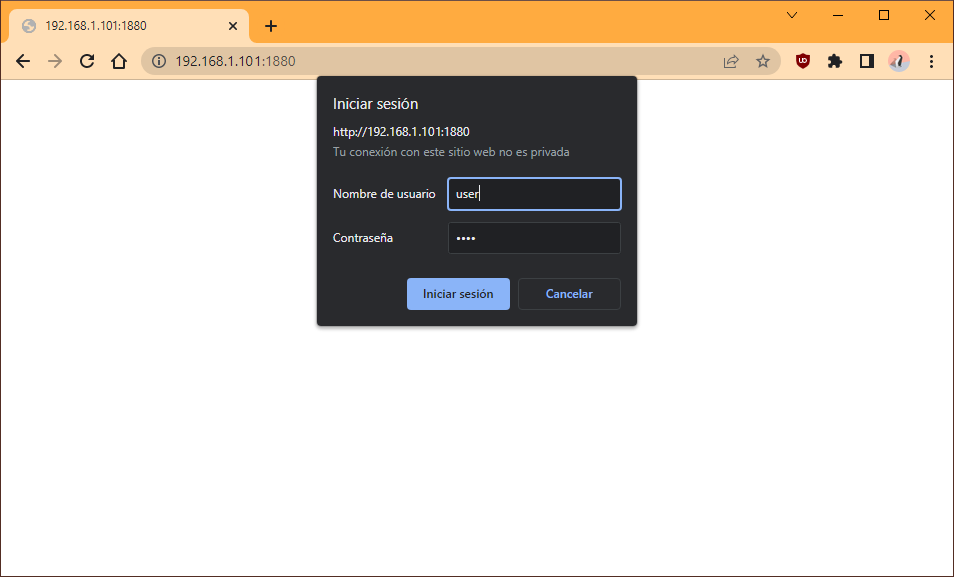
\includegraphics[width=\linewidth]{ImagenesValidacion del prototipo/t-ram-seg-01-1}		
			\caption{Autenticación de usuario para la interfaz gráfica.}
        \end{subfigure}\hfill
        \begin{subfigure}{0.49\textwidth}
        	\centering
        	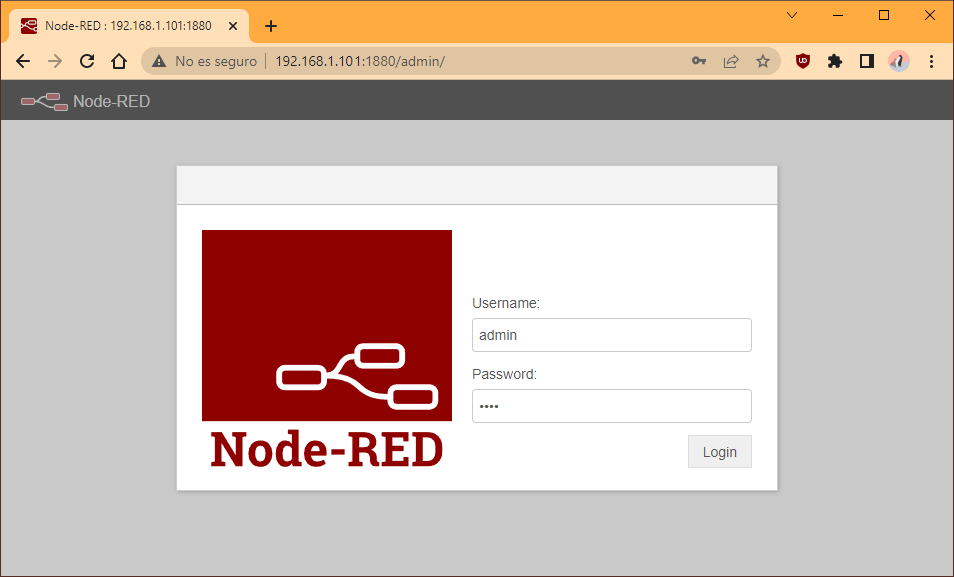
\includegraphics[width=\linewidth]{ImagenesValidacion del prototipo/t-ram-seg-01-2}
        	\caption{Autenticación de administrador para la interfaz gráfica.}
        \end{subfigure}
	\caption{Validación de seguridad \textit{T-RAM-SEG-01}.}
\end{figure}

